\chapter{Time Plan}

The period for the entire project is five months. Suppose our thesis begins on the 15th. April, then the submission deadline is the 15th. September. To ensure the delivery of the project with good quality, a time plan should be developed to arrange the tasks that should be performed during these five months. The tasks should be distributed fairly within the project period so that the tasks can be accomplished with caution and precision.

The tasks for the projects can be divided into three phases and each phase contains one or several parts: \textbf{(I) Implementing the state-of-art approach}:  \textbf{(1.1)} Pre-processing of the input documents, where the input documents are separated into sentences, and the part-of-speech tagging is performed.  \textbf{(1.2)} Information extraction, where we will focus on extracting further information from the sentences. This part is significant work for the whole approach. During this step, the active/passive voice issue will be addressed; the anaphora problem will be solved; the conditional markers will be detected; and all other necessary steps will be performed in this step. \textbf{(1.3)} Flow generation, where each business activity's interactions are identified and connected. \textbf{(1.4)} Post-processing, where we use the flows to generate a BPMN model and convert it into images. \textbf{(II) modify the approach}: \textbf{(2.1) modify the approach}: \textbf{(2.1)} implement the spreadsheet methods  \textbf{(2.2)} rule-based activities recognition, where we will develop the rules for identifying the business rules in the text documents. \textbf{(III) benchmark with the LLM} and finally \textbf{(VI)} Evaluation and redesign, where we evaluate our approach and make improvements regarding the identified limitations of our approach.

\begin{figure}[h]
    \centering
    \caption{Gantt chart of project implementation}
    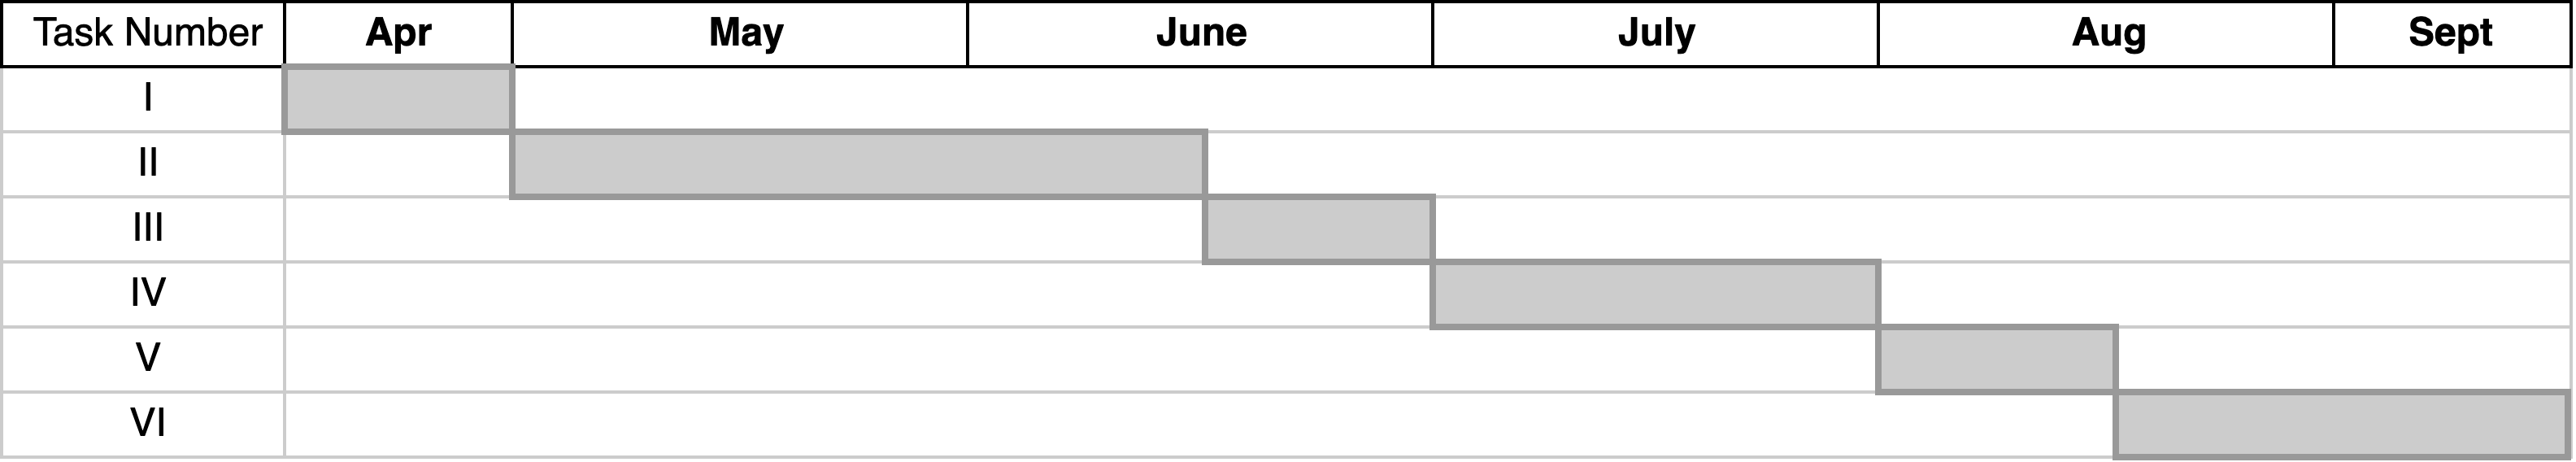
\includegraphics[width=1\textwidth]{tum-resources/images/time_plan.png}
\end{figure}